\documentclass{ximera}
\author{Jont Allen}
\begin{document}
\begin{problem}
    Show that the prime number \(5\) may be factored into Gaussian primes. Hint: Consider \((m + ni)(m - ni)\).
    \[
    \answer{(2 + i)(2 - i)}
    \]
    \begin{feedback}[correct]
    The Gaussian prime factorization of \(5\) is \((2 + i)(2 - i) = 4 + 1\).
    \end{feedback}
\end{problem}

\begin{problem}
    Use MATLAB/Octave to find the prime factors of \(123\), \(248\), \(1767\), and \(999,999\). List the factors from least to greatest:
    \[
    \text{Factors of 123: } \answer{3}, \answer{41}
    \]
    \[
    \text{Factors of 248: } \answer{2}, \answer{2}, \answer{2}, \answer{31}
    \]
    \[
    \text{Factors of 1767: } \answer{3}, \answer{19}, \answer{31}
    \]
    \[
    \text{Factors of 999,999: } \answer{3}, \answer{3}, \answer{3}, \answer{7}, \answer{11}, \answer{13}, \answer{37}
    \]
    \begin{feedback}[correct]
    Use the \texttt{factor()} function in MATLAB/Octave to compute these results.
    \end{feedback}
\end{problem}

\begin{problem}
    Use \texttt{isprime} in MATLAB/Octave to check if \(2\), \(3\), and \(4\) are prime numbers.
    \[
    \text{isprime(2): } \answer{1}
    \]
    \[
    \text{isprime(3): } \answer{1}
    \]
    \[
    \text{isprime(4): } \answer{0}
    \]
    \begin{feedback}[correct]
    The function returns \(1\) for prime numbers and \(0\) otherwise.
    \end{feedback}
\end{problem}

\begin{problem}
    Use the MATLAB/Octave function \texttt{primes} to generate all prime numbers between \(1\) and \(10^6\).
    Save the result in a vector \(x\) and create a histogram of these values using the command \texttt{hist(x)}.
    \begin{multipleChoice}
        \choice[correct]{I've done this.}
        \choice{I have not done this.}
    \end{multipleChoice}
    \begin{feedback}[correct]
    \begin{center}
        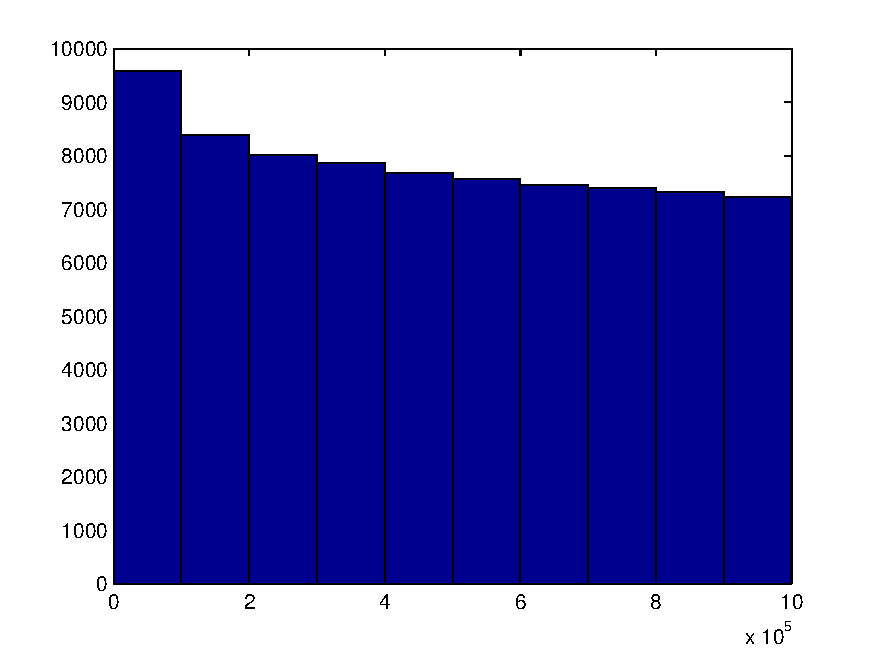
\includegraphics{hw1_2_1c-eps-converted-to.pdf}
    \end{center}
    The function \texttt{primes(10^6)} generates all prime numbers up to \(10^6\). Use the \texttt{hist()} function to visualize the distribution of these numbers. The density of primes decreases as numbers grow larger, following the Prime Number Theorem.
    \end{feedback}
\end{problem}

\end{document}
